\chapter{DBCASE 2.0}
\begin{figure}[H]
    \centering
    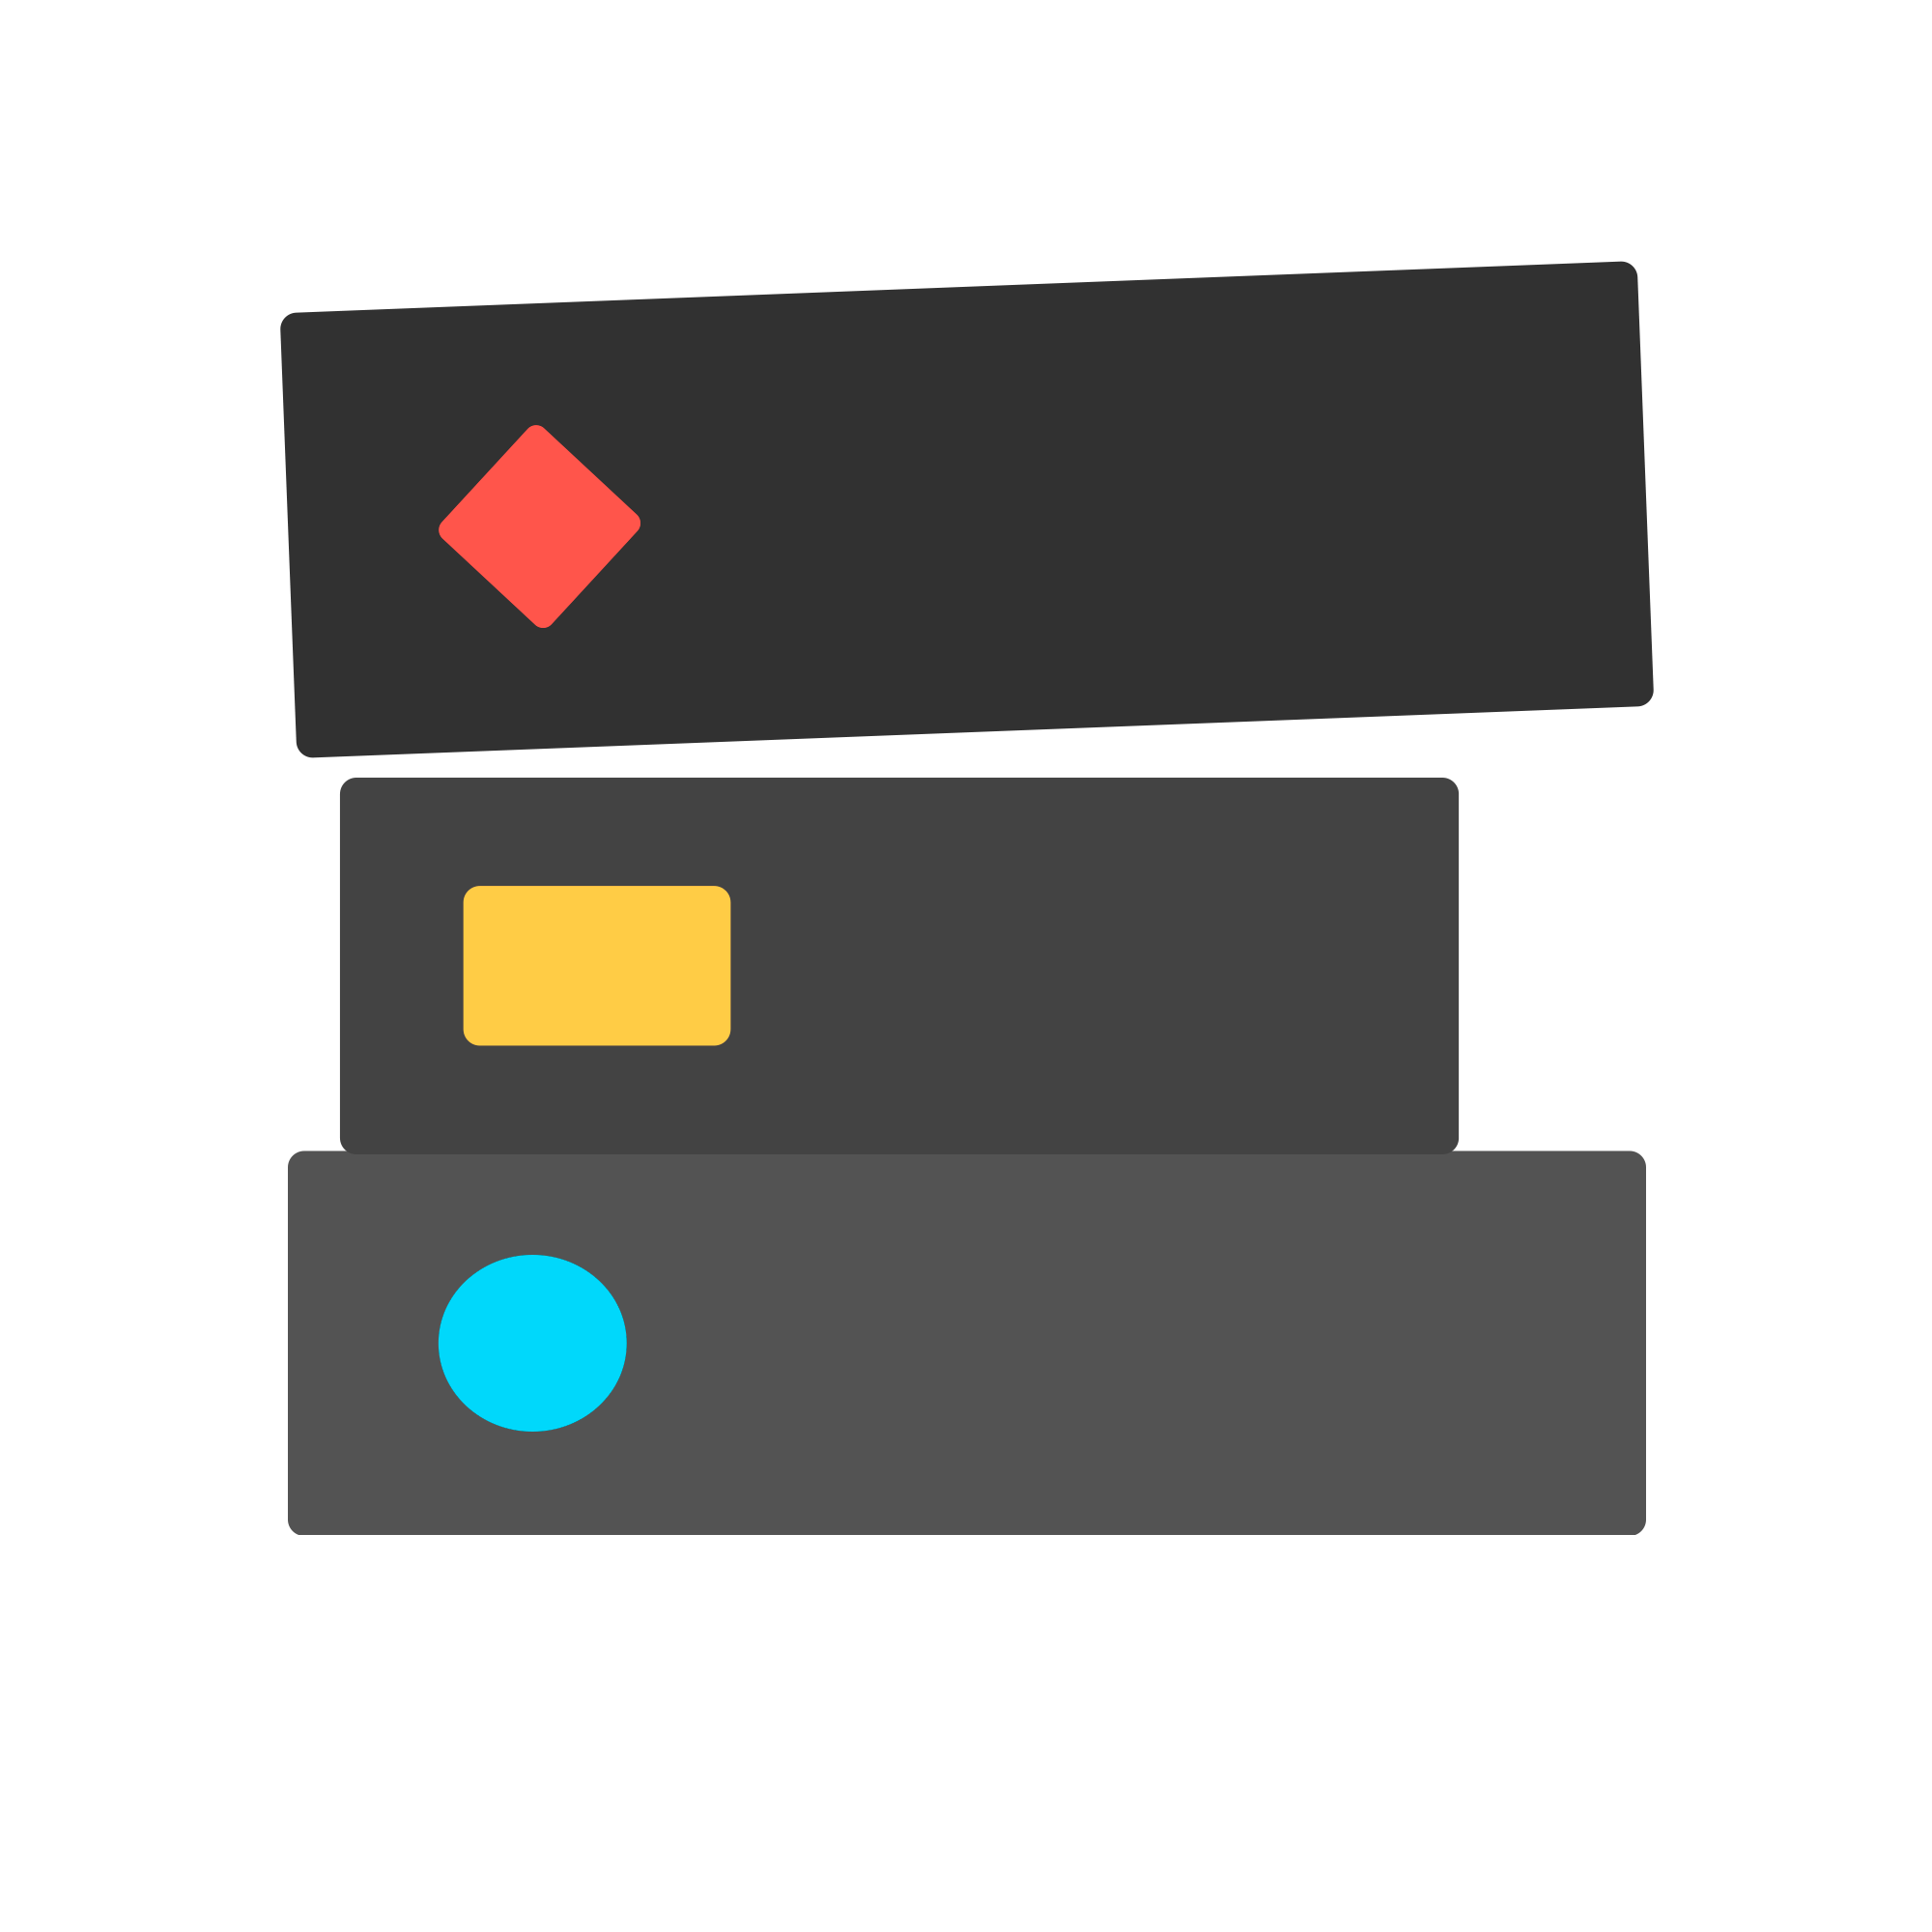
\includegraphics[width=0.5\textwidth]{img/DBCase_logo.png}
\end{figure}
%%
\section{Introducción}
DBCASE 2.0 surge como una actualización al proyecto DBCASE con la que se pretende dar un nuevo aspecto al diseño de la interfaz de usuario y continuar con la implementación de nuevas funcionalidades.\\

El programa está destinado principalmente al uso académico y por ello ha sido pensado como una herramienta didáctica que ayude al alumno en su proceso de aprendizaje, aunque también puede ser usada profesionalmente como una manera fácil y rápida de construir una base de datos relacional. Por ello la herramienta permite al usuario crear una base de datos funcional a partir de un diagrama sin necesidad de que conozca ningún lenguaje de programación de base de datos, lo que es perfecto para alumnos que se estén iniciando en la materia.\\

- Hay que decir que esta hecho en java
%%
\subsection{Antecedentes}
- que se habia hecho en los anteriores proyectos
%%
\subsection{Objetivos}
- actualizar la interfaz
- arreglar los problemas
- 
